\chapter{VLAN}

\section{Overview}

VLANs provide a way to group devices within a LAN. Devices within a VLAN act as if they are in their own independent network, even if they share a common infrastructure with other VLANs. The transmission of unicast, multicast, and broadcast traffic from a host in a particular VLAN are restricted to the devices that are in that VLAN.\\

The primary benefits of using VLANs are as follows:

\begin{itemize}
\item \textbf{Security:} Groups that have sensitive data are separated from the rest of the network, decreasing the chances of confidential information breaches. 

\item \textbf{Better performance:} Dividing flat Layer 2 networks into multiple logical workgroups (broadcast domains) reduces unnecessary traffic on the network and
boosts performance.

\item \textbf{Improved IT staff efficiency:} VLANs make it easier to manage the network because users with similar network requirements share the same VLAN. 
\end{itemize}

There are a number of distinct types of VLANs: 

\begin{itemize}
\item \textbf{Default VLAN:} By default, all switch ports are assigned to default VLAN (VLAN 1). VLAN 1 has all the features of any VLAN, except it cannot be renamed or deleted.

\item \textbf{Native VLAN} is assigned to trunk ports. It serves as a common identifier on opposite ends of a trunk link. It is a best practice to configure a native VLAN for all trunk ports in the switched domain.

\item \textbf{Data VLAN} is configured to carry user-generated traffic. A VLAN carrying voice or management traffic would not be a data VLAN. 

\item \textbf{Management VLAN} is configured to access the management capabilities of a switch. To create the management VLAN, the SVI\footnote{Switch Virtual Interface} of that VLAN is assigned an IP address and a subnet mask. VLAN 1 would be a bad choice for the management VLAN.

\item \textbf{Voive VLAN} is a separate VLAN needed to support Voice over IP (VoIP). 
\end{itemize}

\textbf{Normal range} VLANs are identified by a VLAN ID between 1 and 1005. Configurations are stored within a VLAN database file, called \verb|vlan.dat|. This file is located in the flash memory of the switch. VTP can only learn and store normal range VLANs.\\

\textbf{Extended Range} VLANs are identified by a VLAN ID between 1006 and 4094. Configurations are not written to the \verb|vlan.dat| file, but instead, stored in running configuration file. VTP does not learn extended range VLANs.

\section{VLAN tag}

\subsection{What is tagging?}

A \textbf{trunk} is a point-to-point link between two network devices that carries more than one VLAN. VLAN trunks allow all VLAN traffic to propagate between switches so that devices that are in the same VLAN, but connected to different switches.\\

When Ethernet frames are placed on a trunk, information about the VLANs to which they belong must be added. This process, called \textbf{tagging}, is accomplished by using the IEEE \textbf{802.1Q} header.\\

\begin{figure}[hbtp]
\caption{Fields in Ethernet 801.Q frame}\label{tagging}
\centering
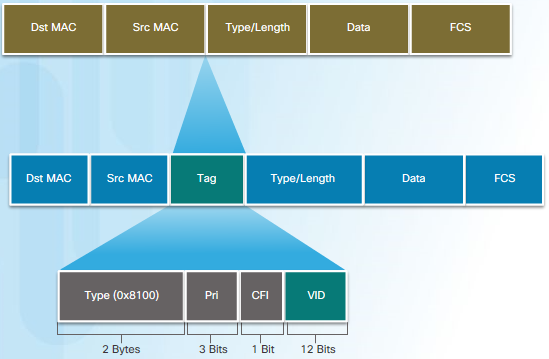
\includegraphics[ width=0.6\textwidth ]{pictures/tagging.PNG}
\end{figure}


The 802.1Q header includes a 4-byte tag inserted within the original Ethernet frame header (Figure \ref{tagging}), specifying the VLAN to which the frame belongs. When the switch receives a frame on an \emph{access} port assigned to a VLAN, the switch inserts a VLAN tag in the frame header, recalculates the FCS\footnote{Frame Check Sequence}, and sends the tagged frame out of a trunk port.\\

\subsection{VLAN tag field}

The VLAN tag field (Figure \ref{tagging}) consists of: 

\begin{itemize}
\item \textbf{Type:} A 2-byte value called the tag protocol ID (TPID) value. For Ethernet, it is set to hexadecimal 0x8100.

\item \textbf{User priority:} A 3-bit value that supports level or service implementation

\item \textbf{Canonical Format Identifier (CFI):} A 1-bit identifier that enables Token Ring frames to be carried across Ethernet links.

\item \textbf{VLAN ID:} A 12-bit VLAN identification number that supports up to 4096 VLAN IDs.
\end{itemize}

After the switch inserts the Type and tag control information fields, it recalculates the FCS values and inserts the new FCS into the frame.

\subsection{Native VLAN and tagging}

A trunk port always forwards untagged frames to the native VLAN. If there are no devices associated with the native VLAN and there are no other trunk ports, then the frame is dropped. Additionally, if an 802.1Q trunk port receives a tagged frame with the VLAN ID that is the same as the native VLAN, it drops the frame.

\subsection{Voice VLAN tagging}

The link between the switch and the IP phone acts as a trunk to carry both voice VLAN traffic and data VLAN traffic. The Cisco IP Phone contains an integrated three-port 10/100 switch. The ports provide dedicated connections to these devices:

\begin{itemize}
\item Port 1 connects to the switch or other VoIP device.
\item Port 2 is an internal 10/100 interface that carries the IP phone traffic.
\item Port 3 (access port) connects to a PC or other device.
\end{itemize}

\begin{figure}[hbtp]
\caption{IP phone ports}\label{PhonePort}
\centering
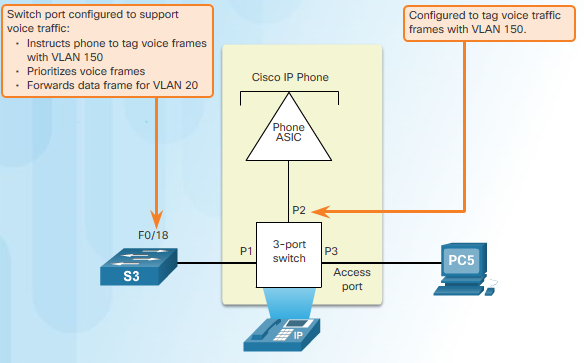
\includegraphics[ width=0.6\textwidth ]{pictures/PhonePort.PNG}
\end{figure}


On the switch, the access is configured to send CDP packets that instruct an attached IP phone to send voice traffic to the switch in one of three ways:

\begin{itemize}
\item In a voice VLAN tagged with a Layer 2 CoS\footnote{Class of Service} priority value
\item In an access VLAN tagged with a Layer 2 CoS priority value
\item In an access VLAN, untagged (no Layer 2 CoS priority value)
\end{itemize}

\section{Configuration}

\subsection{Create VLAN}

A VLAN is created using the \verb|vlan vlan_id| global configuration command. This creates the VLAN and enters VLAN configuration mode. The VLAN can now be assigned a unique name using the \verb|name vlan_name| command.

\begin{verbatim}
S1(config)# vlan 20
S1(config)# name Student
\end{verbatim}

Instead of creating one VLAN at a time, several VLANs can be created using one command. A series of VLAN IDs can be entered separated by commas, or a range of VLAN IDs can be entered separated by hyphens (-). 

\begin{verbatim}
S1(config)# vlan 100,102,105-107
\end{verbatim}

\subsection{Access port}

After creating a VLAN, the next step is to assign access ports to the VLAN. First of all, the port must be assigned as an
access port using the \verb|sw mode access| interface configuration command. Next, assign the port to a VLAN using the \verb|sw access vlan vlan_id| interface configuration command. Note that an access port can belong to only one VLAN at a time.

\begin{verbatim}
S1(config)# interface FastEthernet0/1
S1(config-if)# sw mode access
S1(config-if)# sw access vlan 20
S1(config-if)# end
\end{verbatim}

\subsection{Delete VLAN}

We can delete a VLAN with \verb|no vlan vlan_id| in global configuration mode. However, be careful when removing a VLAN. Before deleting a VLAN, reassign all member ports to a different VLAN. Any ports that are not moved to an active VLAN are unable to communicate with other hosts after the VLAN is deleted. \\

The entire VLAN configuration can be erased using \verb|delete vlan.dat|. This command, along with \verb|erase startup| effectively places the switch into its factory default condition.

\subsection{Trunk port}

To configure a switch port on one end of a trunk link, use the \verb|sw mode trunk| interface configuration command. The native VLAN can also be changed (other than VLAN 1) using \verb|sw trunk native vlan vlan_id|. Always configure both ends of a trunk link with the same native VLAN. \\

Use \verb|sw trunk allowed vlan vlan-list| command to specify the list of VLANs to be allowed on the trunk link.\\

\begin{verbatim}
S1(config)# interface f0/1
S1(config-if)# sw mode trunk
S1(config-if)# sw trunk native vlan 99
S1(config-if)# sw trunk allowed vlan 10,20,30,99
S1(config-if)# end
\end{verbatim}

This configuration assumes the switches automatically use 802.1Q encapsulation on trunk links. Some switches may require manual configuration of the encapsulation. We have to configure 802.1Q encapsulation before trunking mode. Otherwise, the following message will appear:

\begin{verbatim}
Command rejected: An interface whose trunk encapsulation is "Auto" can not be configured to "trunk" mode. 
\end{verbatim}

Whenever this error message appears, use the following solution:

\begin{verbatim}
S1(config)# interface f0/1
S1(config-if)# sw trunk encapsulation dot1q 
S1(config-if)# sw mode trunk
\end{verbatim}

To reset a trunk to allow all VLANs, use the \verb|no sw trunk allowed vlan| interface configuration command. To reset the native VLAN to VLAN 1, use the \verb|no sw trunk native vlan| interface configuration command. To set the port to a non-trunking port, use the \verb|sw mode access| interface command.\\

\subsection{Voice VLAN}

Consider the topology in Figure \ref{VoiceVLAN}. In this example, PC5 is connected to the Cisco IP phone, which in turn is connected to the F0/18 interface on S3. To implement this configuration, Data VLAN 20 (for PC) and Voice VLAN 150 (for IP phone) are created. 

\begin{verbatim}
S3(config)# vlan 20
S3(config-vlan)# name Student
S3(config-vlan)# vlan 150
S3(config-vlan)# name Voice
S3(config-vlan)# exit
S3(config)# 
S3(config)# interface f0/18
S3(config-if)# sw mode access
S3(config-if)# sw access vlan 20
S3(config-if)# 
S3(config-if)# mls qos trust cos
S3(config-if)# sw voice vlan 150
S3(config-if)# end
\end{verbatim}

\begin{figure}[hbtp]
\caption{Sample topology with IP phone}\label{VoiceVLAN}
\centering
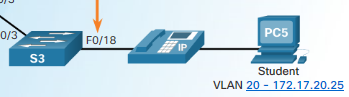
\includegraphics[scale=0.6]{pictures/VoiceVLAN.PNG}
\end{figure}

The command \verb|mls qos trust cos| enables QoS classification based on the class of service (CoS) assigned by the IP phone. The command \verb|sw voice vlan 150| assigns  voice VLAN 150 to port F0/18. 

\subsection{Verification}

VLAN configurations can be validated using the following command:

\begin{verbatim}
S1# show vlan [brief | id vlan-id | name vlan-name | summary]

S1# show vlan name student
S1# show vlan summary
S1# show vlan brief
S1# show interfaces vlan 20
\end{verbatim}

The trunking configuration is verified with the \verb|show int <int> switchport| or \verb|show int trunk|.

\subsection{Troubleshoot}

\paragraph{IP address} Each VLAN must correspond to a unique IP subnet. If two devices in the same VLAN have different subnet addresses, they cannot communicate. This is a common problem, and it is easy to solve by identifying the incorrect configuration and changing the subnet address to the correct one.

\paragraph{Missing VLAN} Verify whether the port is in the correct VLAN using \verb|show vlan| and \verb|show mac address-table int <int>|. Verify if the VLAN is present in the VLAN database using \verb|show vlan|. Use the \verb|show interfaces switchport| command to verify if the inactive VLAN is assigned to the port.


\paragraph{Native VLAN mismatches} Trunk ports are configured with different native VLANs. This configuration error generates console notifications and can cause inter-VLAN routing issues. To solve the native VLAN mismatch, configure the native VLAN to be the same VLAN on both sides of the link.

\paragraph{Trunk mode mismatches} One trunk port is configured in a mode that is not compatible for trunking on the corresponding peer port. This configuration error causes the trunk link to stop working. Be sure both sides of the trunk are configured with the \verb|sw mode trunk| command. 

\paragraph{Allowed VLANs} The list of allowed VLANs on a trunk has not been updated with the current VLAN trunking requirements. 

\section{Inter-VLAN Routing}

Layer 2 switches have limited IPv4 and IPv6 functionality and cannot perform the routing between VLANs. Any device that supports Layer 3 routing, such as a router or a Layer 3 switch (multiplayer), can be used to perform VLAN routing. Regardless of the device used, the process of forwarding network traffic from one VLAN to another is known as inter-VLAN routing. There are three options for inter-VLAN routing: Legacy inter-VLAN routing, Router-on-a-stick, Layer 3 switching using SVIs.

\subsection{Legacy inter-VLAN routing}

In this legacy approach, inter-VLAN routing is performed by connecting different physical router interfaces to different physical switch ports. The switch ports connected to the router are placed in access mode, and each physical interface is assigned to a different VLAN.

\subsection{Router-on-a-stick}

Router-on-a-stick uses a single physical interface to route traffic between multiple VLANs. The router interface is configured to operate as a trunk link and is connected to a switch port that is configured in trunk mode. \\

Router-on-a-stick performs inter-VLAN routing by accepting VLAN-tagged traffic coming from the switch, and then, \emph{internally} routing between the VLANs using subinterfaces. Subinterfaces are virtual interfaces, associated with a single physical interface. Each subinterface is independently configured with an IP address and VLAN assignment (Figure \ref{InterVLAN}). The IPv4 address of the subinterface acts as the default gateway for all hosts in the corresponding VLAN.\\

\begin{figure}[hbtp]
\caption{Router-on-a-stick topology}\label{InterVLAN}
\centering
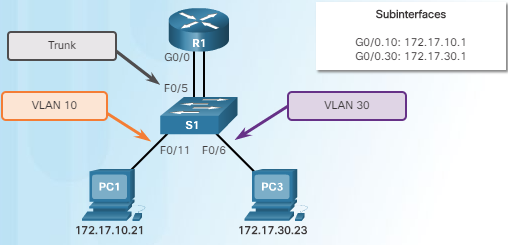
\includegraphics[scale=1]{pictures/InterVLAN.PNG}
\end{figure}


To enable Router-on-a stick, start by enabling trunking on the switch port that is connected to the router.

\begin{verbatim}
S1(config-vlan)# interface f0/5
S1(config-if)# switchport mode trunk
S1(config-if)# end
\end{verbatim}

As for the router, create a subinterface for each VLAN. Then configure 802.1Q trunk for a specific VLAN using \verb|encapsulation dot1q vlan_id|. Next, assign the IPv4 address corresponding to the VLAN subnet. Finally, the physical interface must be enabled. 

\begin{verbatim}
R1(config)# interface g0/0.10
R1(config-subif)# encapsulation dot1q 10
R1(config-subif)# ip address 172.17.10.1 255.255.255.0
R1(config-subif)# 
R1(config-subif)# interface g0/0.30
R1(config-subif)# encapsulation dot1q 30
R1(config-subif)# ip address 172.17.30.1 255.255.255.0
R1(config-subif)# exit
R1(config)# 
R1(config)# interface g0/0
R1(config-if)# no shutdown
\end{verbatim}

\note Use the command \verb|encapsulation dot1q vlan_id native| for the native VLAN. If the \verb|native| keyword option is excluded, the router would consider VLAN 1 as the native VLAN.\\

On the router, use \verb|show vlan| and \verb|show ip route| to verify inter-vlan configuration.

\subsection{Layer 3 switching using SVIs}

Most modern enterprise networks use multilayer switches to achieve much higher packet-switching throughputs (millions of packets per second). Layer 3 switching is much faster than router-on-a-stick, because everything is hardware switched and routed. Despite its price, multilayer switch provide lower latency, support EtherChannel to get more bandwidth. Furthermore, with the multiplayer switch, the network architecture (Figure \ref{NetArch}) is not dependent on STP\footnote{Spanning Tree Protocol, see also section \ref{sec:STP} } anymore because layer 2 loops never occurs in the topology.

\begin{figure}[hbtp]
\caption{Network architecture with multiplayer switches}\label{NetArch}
\centering
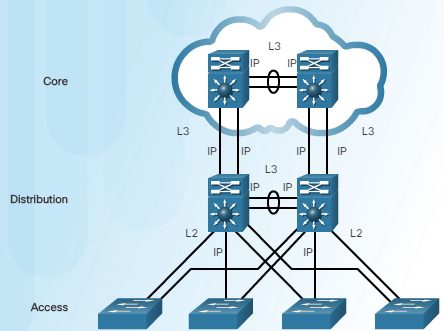
\includegraphics[scale=0.6]{pictures/NetArch.PNG}
\end{figure}


\begin{figure}[hbtp]
\caption{Router-on-a-stick and Multiplayer switch}\label{Layer3sw}
\centering
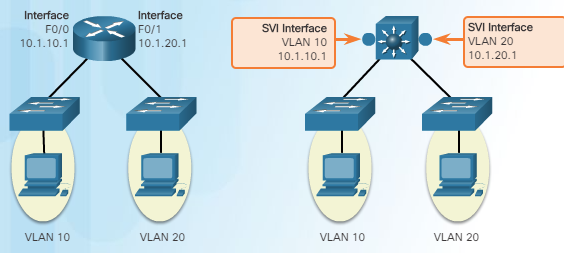
\includegraphics[scale=0.6]{pictures/Layer3sw.PNG}
\end{figure}


Inter-VLAN routing is performed using SVIs and routed ports.
\begin{itemize}
\item \textbf{Routed port:} A pure Layer 3 interface similar to a physical interface on a router. A routed port is not associated with any VLAN. Routed ports are normally implemented between the distribution and the core layer (usually between multiplayer switch and a router or a security device). To configure routed ports, use the \verb|no switchport| interface configuration mode command.

\item \textbf{SVI:} An SVI is configured for each VLAN that exists on the switch. It can perform the same functions as subinterface in Router-on-a-stick method (Figure \ref{Layer3sw}). 
\end{itemize}

\begin{figure}[hbtp]
\caption{Sample topology}\label{Layer3topology}
\centering
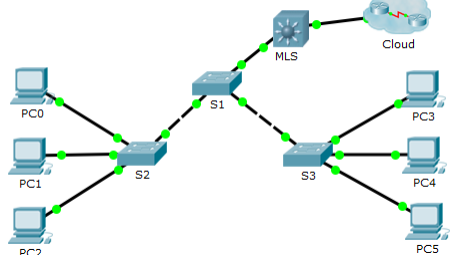
\includegraphics[scale=0.6]{pictures/Layer3topology.PNG}
\end{figure}

Take the multiplayer switch MLS in Figure \ref{Layer3topology} as an example. The first thing to do is enabling layer 3 routing:

\begin{verbatim}
MLS(config)# ip routing
\end{verbatim}

Next, configure G0/2 (connect to the Cloud) as a routed port and assign an IP address:

\begin{verbatim}
MLS(config)# interface g0/2
MLS(config-if)# no switchport
MLS(config-if)# ip address 209.165.200.225 255.255.255.252
\end{verbatim}

Create VLAN 10 and 20, then configure SVI for each of them:

\begin{verbatim}
MLS(config)# vlan 10
MLS(config-vlan)# name Staff
MLS(config-vlan)# exit
MLS(config)# 
MLS(config)# interface vlan 10
MLS(config-if)# ip address 192.168.10.254 255.255.255.0
MLS(config-if)# exit
MLS(config)# 
MLS(config)# vlan 20
MLS(config-vlan)# name Student
MLS(config-vlan)# exit
MLS(config)# 
MLS(config)# interface vlan 20
MLS(config-if)# ip address 192.168.20.254 255.255.255.0
\end{verbatim}

Finally, use the \verb|show ip route| command to verify routing is enabled:

\begin{verbatim}
MLS# show ip route
<output omitted>
C 192.168.10.0/24 is directly connected, Vlan10
C 192.168.20.0/24 is directly connected, Vlan20
  209.165.200.0/30 is subnetted, 1 subnets
C 209.165.200.224 is directly connected, GigabitEthernet0/2
\end{verbatim}